\section{Problemas Mal Condicionados}

São problemas resolvíveis cujas soluções podem ser bastante imprecisas devido a erros de arredondamento.

Por exemplo,

\[
 \left\{
 \begin{array}{rrrrl}
  0.12065\,x & + & 0.98775\,y & = & 2.01045 \qquad \mbox{(A)} \\
  0.12032\,x & + & 0.98755\,y & = & 2.00555 \qquad \mbox{(B)} \\
 \end{array}
 \right.
\]

\textbf{OBS:} (A) e (B) são bem parecidas

\[
\begin{array}{l}
 x_1 = 14.7403 \\
 y_1 = 0.23942
\end{array}
\]

Simulando um erro nos coeficientes da equação (A)

\[
 2.01045 \rightarrow 2.01045 + 0.001 = 2.01145
\]

\[
 \left\{
 \begin{array}{rrrrl}
  0.12065\,x & + & 0.98775\,y & = & 2.01045 \qquad \mbox{(A')} \\
  0.12032\,x & + & 0.98755\,y & = & 2.00555 \qquad \mbox{(B)} \\
 \end{array}
 \right.
\]

\[
\begin{array}{l}
 x_2 = 17.9756 \\
 y_2 = -0.15928
\end{array}
\]

\textbf{OBS:}

\begin{itemize}

\item Pequenas mudanças em outros coeficientes causam mesmo tipo de comportamento.

\item Erros de arredondamento nos coeficientes podem ocorrer durante o próprio processo de solução.

\end{itemize}

\begin{figure}[htb]
 \centering
 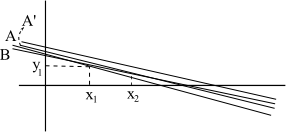
\includegraphics[scale=0.8]{capitulos/capitulo4/figuras/prob_mal_cond1.png}
 \caption{?}
 \label{fig:prob_mal_cond1}
\end{figure}

\textbf{Notas:}

\begin{enumerate}

\item A matriz dos coeficientes de um problema mal condicionado apresenta os seguintes sintomas:

\begin{enumerate}

\item $ a_{ij} + \delta^{ \, \mbox{\tiny{PEQUENO}}} \rightarrow x_k + \Delta^{ \, \mbox{\tiny{GRANDE}}} $

\item $ a_{ii} < a_{kj} $, $ k \neq j $ \, (geralmente)

\item $ det [A] \, det[A]^{-1} \neq 1 $ \, $ (1 \pm \Delta) $

\item $ [A^{-1}]^{-1} \neq A $

\item $ A \, A^{-1} \neq I $

\item $ A^{-1} \, (A^{-1})^{-1} $ \, mais diferente de $I$ do que $ A \, A^{-1} $

\end{enumerate}

\item Pivotação melhora a precisão se o problema for ``moderadamente'' mal condicionado.

\item O melhor procedimento é tentar aumentar ao máximo a precisão (\textit{double})

\[
 \begin{array}{ll}
   \mbox{\textit{Cray}} & \rightarrow \mbox{Precisão simples 8 \textit{bytes} (64 \textit{bits})}\\
   			& \rightarrow \mbox{Precisão dupla 16 \textit{bytes} (128 \textit{bits})}
 \end{array}
\]

\end{enumerate}

\textbf{OBS:} \textit{Singular Value Decomposition of a Matrix}

{
\Large{
\[
 [A_{m \times n}] = [U_{m \times n}] \, [W_{n \times n}] \, [V_{n \times n}]^T
\]
}
}

$U$ e $V$ são matrizes cujas colunas são ortonormais:

\[
 \displaystyle \sum_{i=1}^m U_{ik} \, U_{ij} = \delta_{kj} \, \,
 \left\{
 \begin{array}{l}
   1 \leq k \leq n\\
   1 \leq j \leq n
 \end{array}
 \right.
\]

\[
 \displaystyle \sum_{i=1}^n V_{ik} \, V_{ij} = \delta_{kj}  \, \,
 \left\{
 \begin{array}{l}
   1 \leq k \leq n\\
   1 ? j ? n
 \end{array}
 \right.
\]

{
 \Large{
 \begin{center}
 $
  [A_{n \times n}]^{-1} = [V] \, ${\footnotesize{$
 \left[
 \begin{array}{ccc}
   \ddots & &\\
   & 1/w &\\
   & & \ddots
 \end{array}
 \right]
 $
 }}
 $
 \, [U]^T
 $
 \end{center}
}
}

$c = $ \textit{condition number} $ = \displaystyle \frac{Max(w_i)}{Min(w_i)}$

\begin{itemize}

\item Se $c$ for infinito $ \Rightarrow A$ é singular.

\item Se $c$ muito grande $ \Rightarrow A$ é mal condicionada.

\begin{itemize}

\item muito grande $ \Rightarrow \displaystyle \frac{1}{c} \approx
\left\{
\begin{array}{ll}
 10^{-6} & \mbox{Precisão simples}\\
 10^{-12} & \mbox{Precisão dupla}
\end{array}
\right.
$

\end{itemize}

\end{itemize}
